\documentclass[tikz,border=5mm]{standalone}
\begin{document}
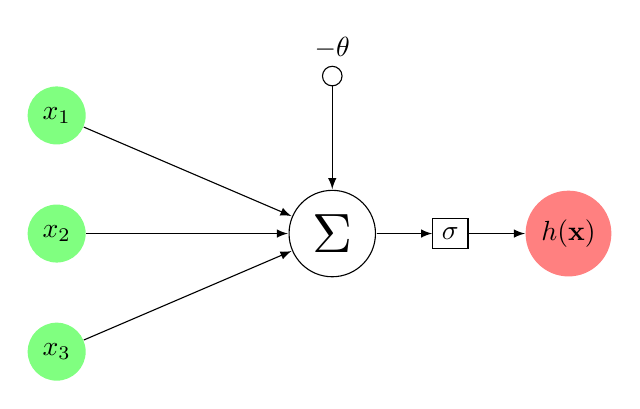
\begin{tikzpicture}[>=latex]
\path
(0,0)     node[circle,draw,scale=2,inner sep=2pt] (S) {$\Sigma$}
+(90:2) node[circle,draw,inner sep=2.5pt] (b) {}
          node[above=1mm] {$-\theta$}
+(-3.5,1.5)  node[circle,fill=green!50]  (x1) {$x_1$}
+(-3.5,0)    node[circle,fill=green!50]  (x2) {$x_2$}
+(-3.5,-1.5) node[circle,fill=green!50]  (x3) {$x_3$}
+(1.5,0)    node[draw] (sigma) {$\sigma$} node[above=3mm]{}
+(3,0)  node[circle,fill=red!50]  (y) {$h(\textbf{x})$};
\draw[->] (S)--(sigma);
\draw[->] (b)--(S);
\draw[->] (x1)--(S) node[pos=.4,above]{};
\draw[->] (x2)--(S) node[pos=.4,above]{};
\draw[->] (x3)--(S) node[pos=.4,above]{};
\draw[->] (sigma)--(y);
\end{tikzpicture}
\end{document}
